
% \paragraph{} This chapter will cover the topics essential to understanding the rationale and implementation of the design as discussed in §~\ref{sec:design}. These include; an introduction to \textit{Information Flow Control} (\textit{IFC}), the Intel SGX platform, and an overview of key aspects of the Linux kernel relevant to the architecture of the prototype.


% -------------

\section{Information Flow Control}
\label{sec:ifc}

\paragraph{} \acrshort{ifc} regulates how and where data is permitted to move and be transformed in a computer system.~\cite{ifc-data-prop} This differs from access control, which defines \textit{what} resources may be used by an entity --- \acrshort{ifc} allows granular control over \textit{how} they may be used once accessed, including restricting propagation between components. 

\paragraph{} Formally, \acrshort{ifc} defines and enforces a non-interference policy between abstract \textit{security contexts}. A simple example is the distinction between \textit{unclassified} and \textit{classified} data --- here, information is only allowed to flow \textit{up}, ensuring that an \textit{unclassified} entity does not learn anything marked as \textit{classified}.~\cite{Bell1973SecureCS} This relationship can generally be represented as a partial ordering over \textit{security contexts}, formulated as a lattice.~\cite{ifc-lattice}

\paragraph{} However, practical systems often require dataflow adhering to a more complicated policy set --- for example, supporting \textit{declassification}.~\cite{10.5555/794199.795122} Work undertaken by Pasquier et al.,~\cite{camflow} the core influence of the \acrshort{ifc} model developed in this project, constructs a pliable and efficient \textit{decentralised \acrshort{ifc}} (\acrshort{difc}) model suitable for provenance enforcement and auditing in the Linux kernel.

\subsection{Motivation, History, and \textit{Decentralised IFC}}

\paragraph{} \acrshort{ifc} has recently grown in popularity as a powerful methodology for ensuring granular privacy whilst not unduly restricting access to sensitive information. \acrshort{ifc} annotates data records with opaque \textit{labels} referring to their confidentiality or integrity status. Rather than simply restricting access to sensitive data, as an access control mechanism would, \acrshort{ifc} tracks data as it propagates --- if an entity attempts to move data into an unknown, untrusted, or conflicting \textit{security context} the \acrshort{ifc} system prohibits this to prevent improper release.

\paragraph{} \acrshort{ifc} originated in the mid-1970s~\cite{ifc-lattice} but has not yet seen mainstream adoption. This may be because early schemes were designed around the \textit{\acrfull{mls}} doctrine set out in the \textit{Orange Book}:~\cite{orange-book} this locked \acrshort{ifc} to a shallow set of broad labels, mirroring existing institutional segregation (such as \textit{restricted}, \textit{secret}, \textit{top secret}). Policies were managed centrally, something easily applicable in settings with rigorous hierarchies such as the military, but unwieldy in an organisation with manifold security protocols.

\paragraph{} The majority of recent research has advocated \textit{decentralised information flow control} 
(\acrshort{difc}), introduced by Myers and Liskov.~\cite{difc,10.1145/363516.363526,10.1145/268998.266669} \acrshort{difc} is more granular than schemes adhering to the \textit{\acrshort{mls}} model, for example, creating two distinct \textit{security contexts} for two files in the same folder. Policies are \textit{discretionary}, allowing users to specify and modify the enforced policies for assets they own.

\subsection{Security Labels and the Reference Monitor}

\paragraph{} A \acrshort{difc} system relies on \textit{tags} and \textit{labels} to annotate the entities it tracks. Let $\mathcal{T}$ be a large set of opaque tokens, or \textit{tags}. Tags are themselves meaningless, but used as an abstract identifier for an entity's \textit{security context}. A \textit{label}, $l \subseteq \mathcal{T}$, is a collection of tags that are concretely attached to assets, such as files; these form a lattice under the subset-relation partial order. For each process $a$ there are two labels, one for secrecy, $a_s$, and one for integrity, $a_i$. For a tag $t$, $t \in a_s$ implies, conservatively, that process $a$ has seen information associated with tag $t$. Likewise, $t \in a_i$ indicates that every input to $a$ has been endorsed for an integrity level marked with $t$.

\paragraph{Walkthrough --- Secrecy Enforcement} In a typical environment, a user can only convince themselves that a text editor is safe to use if they, or someone they trust, audits the program's source code. Using \acrshort{difc}, however, one can reason that a system cannot leak data without permission if the following holds;

\begin{enumerate}
    \item If a process $a$ read a file with a secrecy tag $t$, then $t \in a_s$.
    \item $t \in a_s$ implies that $a$ cannot communicate with another process, $b$, where $t \notin b_s$.
    \item $a$ cannot remove $t$ from $a_s$ without permission.
    \item $t \in a_s$ restricts $a$'s access to an uncontrolled medium, such as a network.
\end{enumerate}

\paragraph{} The heart of an \acrshort{ifc} implementation is its \textit{reference monitor}, which tracks the labelling for each process, granting or rejecting permission before an operation is executed by the \acrshort{os}. Contrasting solutions handle this process differently --- \textit{Flume},~\cite{flume} implements a full system interposition layer, forcing all \textit{syscalls} to pass through its userspace \textit{reference monitor} before reaching the \acrshort{os}, whereas \textit{CamFlow}~\cite{camflow} embeds its \textit{reference monitor} in the kernel itself. In all schemes, however, this trusted component is responsible for both policy and enforcement. This project focusses on this implementation.


\subsection{Modelling}
\label{sec:ifc-modelling}

\begin{table}
    \centering
    \newcommand\tableTop{\rule{0pt}{3ex}}
    \newcommand\tableMid{\rule{0pt}{3ex}}
    \newcommand\tableBottom{\rule[-2ex]{0pt}{0pt}}
    \begin{tabular}{r p{10cm}} 
        \hline
        Notation & Explanation \\ [0.1ex] 
        \hline
            \tableTop{$A \rightarrow B$} & \tableTop{Rule $\alpha$; a permissible information flow between entity $A$ and entity $B$.} \\
            
            $A \Rightarrow B$ & \tableMid{Rule $\beta$; a creation flow, initialising $B$ from $A$ as its parent.} \\

            $A \rightsquigarrow A'$ & \tableMid{Rule $\gamma$; a context change, with $A$ modifying its security context in accordance with its capabilities.} \\
            
            $A \xhookrightarrow[]{t^{\pm}_{x}} B$ & \tableMid{Rule $\delta$; priviledge delegation, with $A$ passing a capability $t_{x}^{\pm}$ to $B$.} \tableBottom \\
    \end{tabular}
    % \vspace{5mm}
    \caption[Overview of the four core IFC events]{Overview of the four core \acrshort{ifc} events used in §~\ref{sec:ifc-modelling}.}
    \label{table:ifc-notation}
\end{table}


\paragraph{} In centralised \acrshort{ifc} schemes, the \textit{reference monitor} is the only entity capable of creating, changing, and assigning tags. However \acrshort{difc} gives \textit{all} processes the ability to create and modify tags for entities they own; thus, they alone have the right to declassify them.

\paragraph{Notation} As the model we build in §~\ref{sec:design} is closest in spirit to \textit{CamFlow}, we use the same notation (Table~\ref{table:ifc-notation}).

\paragraph{Enforcing Safe Flows} ($\alpha$), below, describes the conditions in which a flow can be considered \textit{safe}. The recipient must be \textit{at least as privileged} as the originator and cannot accept information graded below its own integrity status. Here $\preceq$ denotes any applicable preorder relation; this context uses inclusion ($\subseteq$). If a flow is \textit{impermissible} it is denoted as $A \nrightarrow B$.
\begin{equation}
    A \rightarrow B \iff A_s \preceq B_s \;\; \land \;\; B_i \preceq A_i \tag{$\alpha$}
\end{equation}
\vspace{-12mm}

\paragraph{} Information produced within a \textit{security context} may only flow within the same context or a related \textit{subcontext}.

\paragraph{Entity Creation} ($\beta$) shows correct initialisation of a new object's \textit{security context}. Logically it must be held at the same level as the environment creating it. For example, when a process creates a new file, this must subject to the same tainting as the original process.

\vspace{-5mm}
\begin{equation}
    A \Rightarrow B \implies A_s = B_s \;\; \land \;\; A_i = B_i \tag{$\beta$}
\end{equation}

\paragraph{Vocational Label Management} The core mantra of the \textit{decentralised} aspect of \acrshort{difc} is that processes are responsible for policies governing their assets. Therefore, a process's labelling must be dynamic. Generally, entities are sorted into two distinct categories;

\begin{itemize}
    \item \textit{Active} (processes), with \textit{mutable} security contexts.
    \item \textit{Passive} (files, pipes, sockets, etc.), which merely act as data vessels for \textit{active} entities.
\end{itemize}

\paragraph{} \textit{Active} entities may modify their labelling iff they have the capability to add or remove specific tags. The set $A_{s}^{+} \subseteq \mathcal{T}$ lists all the tags that entity $A$ may add to its security labelling, while $A_{s}^{-} \subseteq \mathcal{T}$ holds all the tags $A$ may remove from its labelling. These sets are modified either during creation or in receipt of a delegated capability from a peer. The sets $A_{i}^{\pm} \subseteq \mathcal{T}$ also exist, performing the same function for integrity labels. ($\gamma$) formalised this process.


\begin{equation}
    \left\{\begin{array}{lr}
        A'_x \leftarrow A_x \cup \{t\} & \text{if} \;\; t \in A_{x}^{+} \\
        A'_x \leftarrow A_x \smallsetminus \{t\} & \text{if} \;\; t \in A_{x}^{-} \\
    \end{array}\right\} \implies A \rightsquigarrow A' \tag{$\gamma$}
\end{equation}

\paragraph{} A notable restriction is that processes must be aware of the \acrshort{ifc} constraints imposed on them and how to interact with the system to manage their labels.

\paragraph{Capability Lifecycle and Delegation} As per ($\beta$), an entity automatically inherits the labelling of its creator without any capabilities ($A_{s}^{\pm}, A_{i}^{\pm} = \varnothing$), therefore requiring \textit{capability delegation} ($\delta$). A capability held by $A$, $t_{x}^{\pm}$, where $t \in A_{x}^{\pm}$, is permitted to be transferred to $B$ to act on its behalf.

\vspace{-3mm}
\begin{equation}
    A \xhookrightarrow[]{t^{\pm}_{x}} B \;\; \text{only if} \;\; t \in A_{x}^{\pm} \tag{$\delta$}
\end{equation}

\paragraph{} Delegation is vital for webservers, for example. To transmit another entity's information over an untrusted socket the server must have permission to \textit{declassify} it --- i.e. it must hold $f_{s}^{-}$, where $f$ is the secrecy label of the information to transmit.\footnote{The server process, $W$, must have $W_{i} = \varnothing$ as it holds a connection to an untrusted socket. Thus the integrity clause in ($\alpha$) will not interfere.}


% ---------
\clearpage
\section{Intel® SGX}

\paragraph{} Intel's \acrfull{sgx} was first detailed in 2013.~\cite{10.1145/2487726.2488370, 10.1145/2487726.2488368, Anati2013InnovativeTF, sgx-sgx-reference} Its whitepapers described a novel approach to \textit{trusted computing}, creating in-\acrshort{cpu} containers with dedicated protected memory pools. These regions, called \textit{enclaves}, cannot be read from or written to by an unauthorised party due to fundamental protection mechanisms provided by the x86 architecture, even if running in \textit{ring 0}\footnote{Linux uses two of x86's four protection \textit{rings} --- \textit{0} for the kernel, and \textit{3} for userspace.} (Figure~\ref{fig:sgx-basic}). \textit{Enclaves} guarantee both integrity and secrecy to the application running inside, even in the presence of a malicious host.

\paragraph{Motivation} Broadly, \acrshort{sgx} secures sensitive applications by shielding them and their resources from any access, and to guarantee an enclave's integrity to end-users; this is achieved using attestation and measurement (see §~\ref{sec:attestation}). One use case~\cite{10.1145/2834050.2834100, 10.1145/2799647, 10.1145/2810103.2813695} is in cloud computing, where users are forced to trust an outside party with their data and business logic. By distributing encrypted, yet executable, containers targetted at a single, unique \acrshort{sgx} core, users can be assured that their information is safe, despite virtualisation. Only the provisioned \acrshort{cpu} is able to decrypt and execute the enclave, strictly in accordance with the restrictions of the \acrshort{cpu} platform.

\subsection{Security Characteristics}

\begin{figure}[]
    \centering
    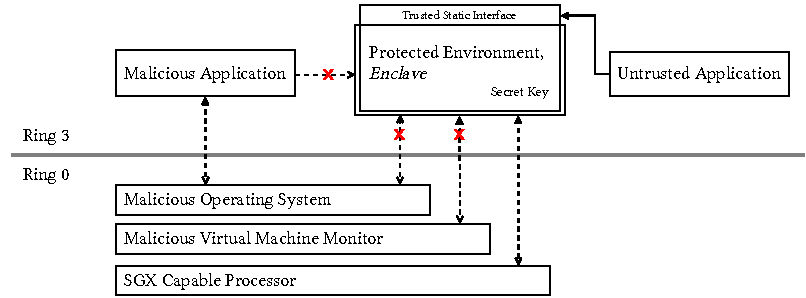
\includegraphics[width=0.95\linewidth]{figures/SGX-architecture.pdf}
    \caption{Abstract overview of SGX's protection in an adversarial environment.}
    \label{fig:sgx-basic}
\end{figure}

\paragraph{} At its heart \acrshort{sgx} is designed to be \textit{trustworthy}; this is achieved in several ways, including robust enclave provisioning, sealing and attestation. Intel summarises \acrshort{sgx}'s protections~\cite{10.1145/2487726.2488368,sgx-eval-sdk} as follows;

\begin{itemize}
    \item Memory is secured against observation and modification from outside the enclave, using an in-die \textit{\acrfull{mee}},~\cite{sgx-mee} with a secret that rotates on every boot. This protection notably works against host hypervisors, other enclaves, and anything running in supervisor mode.
    \item Enclaves can \textit{attest to}, or prove, their identity to a challenger with the help of a permanent hardware security key for asymmetric encryption.
    \item Software calls are proxied to prepare and transfer control in and out of an enclave. Arguments are securely marshalled according to a static enclave definition.
    \item \acrshort{sgx} does not defend against reverse engineering or side-channel attacks:~\cite{10.1109/SP.2015.45} mitigating this is the developer's responsibility.
    % \item Debugging support is only provided via a specialised tool and only when an enclave is compiled with debugging enabled.
\end{itemize}

\subsection{Architecture and Implementation}

\begin{figure}[]
    \centering
    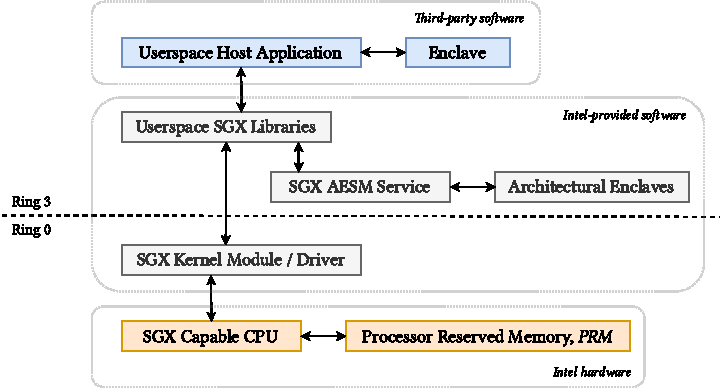
\includegraphics[width=0.9\linewidth]{figures/SGX-AdvArchitecture.pdf}
    \caption{A high-level overview of the SGX hardware and software architecture.}
    \label{fig:sgx-advarch}
\end{figure}

\paragraph{} The \acrshort{sgx} platform comprises several interlocking parts (Figure~\ref{fig:sgx-advarch}), building on the core extended x86 instruction set. Information here as reported by~\cite{sgx-sgx-reference,Costan2016IntelSE}.

\subsubsection{Hardware}
\paragraph{} Enclaves' state is stored securely in \textit{\acrfull{prm}} a set of pages in system memory presided over by the \textit{\acrshort{mee}}. \textit{\acrshort{prm}} consists of two data structures; the \textit{\acrfull{epc}} and the \textit{\acrfull{epcm}}.

\paragraph{} An enclave is defined by its \textit{\acrshort{secs}} --- generated when an enclave is created and stored in a dedicated entry in the \textit{\acrshort{epc}}. A \textit{\acrshort{secs}} holds important metadata including; the enclave's (system-)global identifier, its measurement hash (\texttt{MRENCLAVE}, §~\ref{sec:attestation}) and its memory usage.

\paragraph{} The \textit{\acrshort{epcm}} provides an index into the \textit{\acrshort{epc}}: it stores access control information, ownership and validity indicators, and a marker for a page's designated use --- this is not accessible from software. 

\paragraph{} \textit{\acrshort{prm}} pages are only successfully resolved if the \acrshort{cpu} is in enclave mode and the \textit{\acrshort{epcm}} corroborates the enclave's ownership of the region; invalid requests are presented with an unused page from generic system memory. Direct Memory Access to \textit{\acrshort{prm}} is always rejected.

\paragraph{} The \textit{\acrshort{epc}} is managed by the system's hypervisor or \acrshort{os} as typical memory, but it must use \acrshort{sgx}-specific instructions. This is to appease the \textit{\acrshort{mee}}, which is responsible for ensuring the integrity and confidentiality of this process, encrypting and decrypting pages as they cross the \textit{\acrshort{prm}} boundary. An \acrshort{sgx} driver, \textit{isgx}, is required to allow userspace applications to use the platform and create/manage enclaves.


\subsubsection{Userspace Services}
\paragraph{} Starting an enclave requires retrieving a \textit{launch token} from Intel's \textit{Launch Enclave}; this checks the enclave's validity and identity. Access to the \textit{Launch Enclave} and other architectural enclaves is provided by the \acrfull{aesm}; the userspace \acrshort{sgx} libraries facilitate communication. Other architectural enclaves include;

\begin{itemize}
    \item The \textit{Provisioning Enclave} --- verifies the authenticity of the platform and retrieves an enclave's \textit{attestation key} from the \textit{Intel Provisioning Service's} servers.
    \item The \textit{Quoting Enclave} --- provides trust in the identity of the \acrshort{sgx} environment and enclave being attested, by converting the locally generated \textit{attestation key} to a remotely-verifiable \textit{quote}.
\end{itemize}

\subsubsection{Third-party enclaves}
\paragraph{} Enclaves are always accompanied by a host application which acts as its untrusted counterpart. The host application calls the \acrshort{sgx} \acrshort{sdk} to build an enclave on its behalf using an enclave image, packaged as a standard shared library and returns its \textit{global identifier}. Control is passed from the host application to the enclave by invoking an enclave function via an \textit{ECALL}. Execution flow can temporarily leave the enclave if it calls one of the host application's functions via an \textit{OCALL}. Execution naturally leaves enclave-mode when an \textit{ECALL} terminates. Both \textit{ECALLs} and \textit{OCALLs} are defined statically in the enclave's interface definition (\texttt{enclave.edl}), and the necessary glue code is generated by the \acrshort{sgx} \acrshort{sdk}'s build toolchain at compile time; this ensures calls crossing the enclave boundary are marshalled safely and correctly.


\subsection{Enclave Lifecycle}
\label{sec:sgx-lifecycle}

\paragraph{} \acrshort{sgx}
instructions can be separated into two distinct groups; privileged and unprivileged (Table~\ref{table:sgx-instructions}\footnote{A few instructions irrelevant to the explanation given here are omitted.}). The following description is illustrated in Figure~\ref{fig:sgx-enclavecreate}.

\paragraph{Preparing an enclave} The host application begins initiating the creation process via \textit{isgx}, the \acrshort{sgx} driver. \textit{isgx} allocates the requisite number of pages to run the enclave $\langle 1 \rangle$;\footnote{Numbers correspond to events in Figure~\ref{fig:sgx-enclavecreate}.} this is tracked by the driver's internal state $\langle 2 \rangle$.

\paragraph{} The application next calls \texttt{ECREATE} with the metadata of the enclave to be loaded $\langle 3 \rangle$; the \textit{\acrshort{mee}} checks that the pages being claimed are vacant and populates the \textit{\acrshort{secs}} page $\langle 4 \rangle$. Once complete the application prepares the remaining \textit{\acrshort{epc}} pages using \texttt{EADD} $\langle 5 \rangle$ and loads the enclave's code and data $\langle 6 \rangle$.

\paragraph{} Next the enclave is measured --- \texttt{EEXTEND} is called $\langle 7 \rangle$, triggering the \textit{\acrshort{mee}} to update the measurement hash in the \textit{\acrshort{secs}} to mirror the current state of the enclave's memory $\langle 8 \rangle$. After, the \textit{\acrshort{epc}} memory is finalised using \texttt{EINIT} $\langle 9 \rangle$: this operation requires the application to retrieve the \texttt{EINITTOKEN} from the \textit{Launch Enclave}, locking the execution of the measured enclave to currently assigned processor core. Notably, pages cannot be added after \texttt{EINIT},\footnote{Only strictly true in \acrshort{sgx} v1, see §~\ref{sec:sgx-versions}.} and an enclave cannot be attested to or entered before it. Lastly, the \textit{\acrshort{secs}} is updated with the enclave's final hash $\langle 10 \rangle$.


\begin{figure}[]
    \centering
    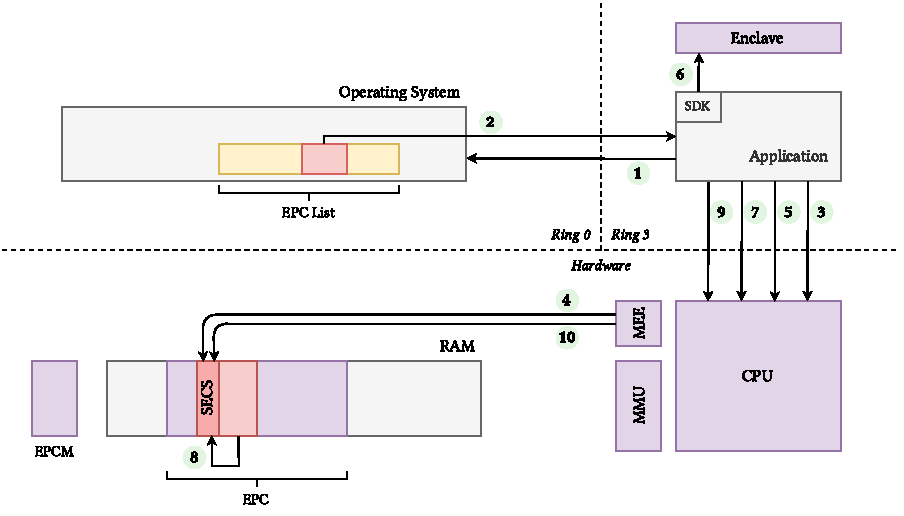
\includegraphics[width=\linewidth]{figures/SGX-EnclaveCreate.pdf}
    \captionsetup{justification=centering}
    \caption[The process of creating and initialising an enclave.]{The process of creating and initialising an enclave; details given in §~\ref{sec:sgx-lifecycle}. Purple components belong to the SGX platform.}
    \label{fig:sgx-enclavecreate}
\end{figure}

\paragraph{Stepping into the enclave} After creation, an enclave may be invoked using the \texttt{EENTER} instruction; this can only jump to points explicitly defined in the enclave's interface definition, and switches the \acrshort{cpu} core to enclave mode. \acrshort{sgx} uses a flag in the \acrshort{cpu} core's \textit{Thread Control Block} to prevent any other logical core following the current one into the enclave.

\paragraph{} Interrupts and exceptions can be served to the enclave, just as with any other application. Control, however, is not immediately passed over to the defined handler. Instead the enclave's current state is saved and cleared to prevent leaking. The \textit{Asynchronous Enclave Exit} routine is then invoked and enclave mode disabled. Execution post-interruption is restarted with \texttt{ERESUME}. Once execution completes, all registers are erased and \texttt{EEXIT} called. Enclaves are terminated using the \texttt{EREMOVE} command; all claimed \textit{\acrshort{epc}} pages are marked as invalid and the \textit{\acrshort{secs}} page deleted.

\paragraph{} \label{sec:sgx-no-kernel-mode} A significant restriction of the \acrshort{sgx} architecture is that enclaves cannot be entered from \textit{ring 0};~\cite{sgx-prog-reference} the required instructions are simply not available. Thus all host applications must run in userspace, making interoperation with the kernel challenging, as discussed in §~\ref{sec:challenges}.

\begin{table}
    \centering
    \newcommand\tableTop{\rule{0pt}{3ex}}
    \newcommand\tableMid{\rule{0pt}{3ex}}
    \newcommand\tableBottom{\rule[-2ex]{0pt}{0pt}}
    \begin{tabular}{|c|r|p{8.5cm}|} 
        \hline
        Execution Mode & Instruction & Function \\ [0.1ex] 
        \hline\hline
        \multirow{11}{*}{Ring 0} 
            & \tableTop{\texttt{ECREATE}} & \tableTop{Generate and copy the \textit{\acrshort{secs}} structure to a new page in the \textit{\acrshort{epc}}, initialising a new enclave.} \\ 
            & \texttt{EADD} & \tableMid{Add a new \textit{\acrshort{epc}} page for the current enclave; this is used to load initial code and data.} \\ 
            & \texttt{EEXTEND} & \tableMid{Update the enclave's measurement during attestation; modifies the \textit{\acrshort{secs}}.} \\ 
            & \texttt{EINIT} & \tableMid{The terminal instruction in an enclave's initialisation, finalising its attributes and measurement.} \\ 
            & \texttt{EREMOVE} & \tableMid{Permanently remove a page from the \textit{\acrshort{epc}}; usually invoked during enclave destruction.} \tableBottom \\ 
        \hline\hline
        \multirow{11}{*}{Ring 3} 
        & \tableTop{\texttt{EENTER}} & \tableTop{Transfer control from the host application to a pre-determined location in an enclave.} \\ 
        & \texttt{ERESUME} & \tableMid{Re-enter the enclave after an interrupt/exception and resume execution.} \\ 
        & \texttt{EEXIT} & \tableMid{Restore the original operating mode at the location \texttt{EENTER} was triggered and flush the \acrshort{tlb}.} \\ 
        & \texttt{EGETKEY} & \tableMid{Access platform cryptography keys required for attestation and sealing.} \\ 
        & \texttt{EREPORT} & \tableMid{Generate a \textit{report} for an enclave's \textit{attestation key} for an attestation process.} \tableBottom \\ 
        \hline
    \end{tabular}
    \vspace{5mm}
    \caption[Overview of notable SGX x86 instructions in an enclave's lifecycle.]{Overview of notable SGX x86 instructions in an enclave's lifecycle.~\cite{sgx-prog-reference}}
    \label{table:sgx-instructions}
\end{table}


\subsection{Attestation}
\label{sec:attestation}

\paragraph{} An essential feature of the \textit{trusted computing} model \acrshort{sgx} creates is attestation, the process of verifying both the authenticity and integrity of components cryptographically. \acrshort{sgx} achieves this by creating two \textit{signing identifiers} per enclave; \texttt{MRENCLAVE} and \texttt{MRSIGNER}.~\cite{Anati2013InnovativeTF,sgx-prov-service}

\paragraph{} \texttt{MRENCLAVE} acts an a unique identifier for enclave's contents. It is generated by hashing the instructions and data passed when creating the enclave with \texttt{ECREATE}, \texttt{EADD}, and \texttt{EEXTEND}; the value is finalised and stored in the \textit{\acrshort{secs}} on \texttt{EINIT}. This value depends on the exact content and ordering of the enclave's \textit{\acrshort{epc}} pages. As long as the enclave's source remains the same, so will its \texttt{MRENCLAVE}.

\paragraph{} \texttt{MRSIGNER}, also known as the enclave's \textit{Sealing Identity}, is generated during the enclave build process --- all production enclaves need to be signed using an \acrshort{rsa} key provided by the compiling user (the \textit{Sealing Authority}). The public key from this pair is stored in \textit{SIGSTRUCT}, the \textit{Enclave Signature Structure}. During an enclave's launch its signed compile-time \texttt{MRENCLAVE} value (held in \textit{SIGSTRUCT}) is decrypted and crossreferenced with a freshly-computed runtime \texttt{MRENCLAVE} value to detect tampering. \texttt{MRSIGNER} is the same for all enclaves signed by the same \textit{Sealing Authority}.

\paragraph{Local Attestation} Two enclaves resident on the same system are able to attest their identities to each other using their \texttt{MRENCLAVE} and \texttt{MRSIGNER} values; this usually precedes the establishment of a shared secret (using a variant of \textit{Diffie-Hellman}~\cite{10.1109/TIT.1976.1055638} backed by the platform's master \acrshort{sgx} key) for confidential communication between them.

\paragraph{Remote Attestation} The Intel specification also enables an enclave to attest its identity to a remote party. The system's \textit{Quoting Enclave} verifies an enclave's local \textit{quote} and creates a digital signature of it using the \acrshort{cpu}'s permanent hardware \acrshort{sgx} private key. Using an \textit{\acrfull{epid}}~\cite{epid} allows this process to complete anonymously, relying on information encoded in the \acrshort{cpu} during manufacturing. The \textit{Provisioning Enclave} assists in this process, especially as production enclaves are required to attest with Intel's provisioning service~\cite{sgx-prov-service} before executing. Remote attestation is not explicitly required in this project, hence will not be covered further.

\subsection{Sealing}
\label{sec:sealing}
\paragraph{} \textit{Sealing} is the encryption of data using a key unique to the generating enclave on a particular platform. \acrshort{sgx} offers two policies for deriving the encryption key based on the platform's \textit{Root Sealing Key} --- relative to the current enclave (\texttt{MRENCLAVE}) or the current enclave's \textit{Sealing Authority} (\texttt{MRSIGNER}). These serve many use cases, including allowing state to persist through enclave upgrades.

\subsection{SGX Versions}
\label{sec:sgx-versions}
\paragraph{} There are currently two versions of \acrshort{sgx} available --- the details given here relate to \textit{v1} as this project will be compatible with both. \textit{v2} offers a number of improvements on which this project does not rely, including: dynamic memory management, eased production enclave restrictions (`Flexible Launch Control'), increased \acrshort{prm} size support, and support for virtualisation.


% -------------

\section{Aspects of the \textit{Linux} Kernel}

\paragraph{} Linux needs little introduction. Created in 1991 as an open-source alternative to UNIX, it now powers over 90\% of \textit{the cloud} and 85\% of smartphones. With almost 25,000 contributors to the kernel, it is immensely complex, with numerous interlocking parts. This section provides a brief overview of a small subset of them to support the design presented in §~\ref{sec:design}.

\subsection{Virtual File System}

\paragraph{} Linux represents almost every component as a file, including sockets, terminals, and driver interfaces. The \acrshort{vfs} is the transparent layer that provides this abstraction, routing requests to the correct underlying implementation. This virtual interface relies on the following mechanisms.

\paragraph{Superblocks} The \textit{superblock} attached to an entity represents the characteristics and properties of the filesystem in which it sits. An important marker held in the superblock is it's \textit{magic value}; this predefined code\footnote{Defined in \texttt{include/uapi/linux/magic.h}.} indicates the underlying implementation the filesystem belongs to.

\paragraph{Inodes} The \textit{inode} data structure represents information about a single file existing on a file system. All objects, not only files, are \textit{backed} by inodes. No pathname is assigned at this level; this is provided at a higher level of abstraction. An inode does however indicate ownership, access restrictions and content type, and is identified by its \textit{inode number}.

\paragraph{Dentries} Each item in the \textit{direct entry cache} (\textit{dcache}), shortened to \textit{dentry}, represents a connection between an inode and its path in the \acrshort{vfs}. This glue layer is responsible for building the tangible folder structure, and as the name suggests, metadata caching. A \textit{file} consists of a \textit{dentry}-\textit{inode} pair.

\paragraph{File descriptors} Whenever a process opens a file, it is presented with a \textit{file descriptor} by the kernel. This structure is unique to a process, providing the gateway between the process and the underlying file it describes. All active descriptors can be viewed at \texttt{/proc/<pid>/fd/}; for standard processes \textit{0} globally refers to \textit{stdin}, \textit{1} to \textit{stdout}, and \textit{2} to \textit{stderr}. Reads and writes to a file (or socket, pipe, etc.) are performed on the relevant file descriptor, not the object directly.

\subsubsection{Extended Attributes} 

\paragraph{} Files can have additional, external, key-value pairs attached to them. These attributes, shortened to \textit{\acrshort{xattr}s}, are permanent and saved to disk alongside the file's content. Values must be in the form of a null-terminated string, however they are optional and may be left empty if the attribute is just a flag. \textit{\acrshort{xattr}s} are namespaced to define different classes of functionality; the \texttt{user} namespace is open to all (e.g. \texttt{user.example\_attribute}), but \texttt{trusted}, \texttt{system}, and \texttt{security} are reserved for specific uses by the kernel --- the \texttt{security} namespace belongs exclusively to \acrshort{lsm}s (§~\ref{sec:lsm}).

\subsubsection{\textit{sysfs}}
\paragraph{} \textit{sysfs} is a pseudo-filesystem provided by the \acrshort{vfs}, that the kernel uses to export its subsystems via a virtual file interface.\footnote{\texttt{/sys}} Specific instantiations of \textit{sysfs} are used for various purposes --- for example, \acrshort{lsm}s and \textit{SecurityFS}.\footnote{\texttt{/sys/kernel/security}}



\subsection{Linux Security Modules}
\label{sec:lsm}

\paragraph{} Linux supports the inclusion of third-party security models in the kernel itself using a unified framework, \acrshort{lsm}. This provides developers with \textit{hooks} into kernel functionality at every point a userspace \textit{syscall} is about to access fundamental kernel primitives, such as inodes or task control structures. Each of these hooks can influence the behaviour of the kernel by allowing or denying the operation.

\paragraph{} \acrshort{lsm} attaches a \texttt{void*} security field to every instance of kernel primitives, such as \texttt{struct inode}, to allow security implementations to attach additional state to each, tracking them as appropriate. Decisions taken within an \acrshort{lsm} affect all aspects of a Linux system; \textit{superuser} privilege cannot override it and every component in the system can be restricted.


\subsubsection{Integrity Measurement Architecture}
\label{sec:ima}

\paragraph{} Linux's \acrshort{ima} subsystem is responsible for calculating the hashes of files and programs as they are loaded (\textit{measurement}), verifying them against an allowed list if required (\textit{appraisal}). Its driving purpose is to detect if files have been maliciously altered remotely or locally; the file's hash is stored as an \textit{\acrshort{xattr}} (\texttt{security.ima}). \acrshort{ima} supports many use cases, the majority of which are complementary to the \acrshort{lsm} framework, but we shall focus on one here --- \acrshort{evm}.

\paragraph{} The Linux \textit{\acrfull{evm}} protects \textit{\acrshort{xattr}s} in the \texttt{security} namespace --- this covers both the \acrshort{ima} hash and any labels created by security modules. Two tamper-detection methods are provided:

\begin{enumerate}
    \item The \textit{HMAC-SHA1} hash of the \texttt{security} namespace is stored, for reference, as \texttt{security.evm}, and
    \item A digital signature of this value is stored alongside using a key that is sealed either using a \textit{Trusted Platform Module}~\cite{tpm} or passphrase.
\end{enumerate}
